\chapter{The CMS detector and the Large Hadron Collider}
\label{c:det}
This chapter discusses the Large Hadron Collider (LHC) which is located on the Franco-Swiss border near Geneva approximately 100 m undergrounds at the site of the Centre European de Research Nuclear (CERN). It is a 26.7 km long synchrotron particle accelerator with four interaction points where four experiments are located.  My thesis focuses on results from the Compact Muon Solenoid detector described in section~\ref{sec:CMSdet}. The other experiments include ATLAS which is a multi-purpose experiment like CMS, the LHCb detector which focusses on the study of the physics of B mesons and the ALICE detector which is used to study quark-gluon plasmas.

\section{LHC}

The LHC accelerates two beams of protons which circulate in opposite directions \fixme{describe opposite magnetic dipoles}. The protons are sourced from a bottle of hydrogen where a strong electric field is used to rip apart the electrons from the hydrogen atom leaving protons behind. The protons are then accelerated through the linear accelerator LINAC2 before being injected into the Proton Synchrotron Booster (PSB), then into the Proton Synchrotron (PS) followed by the Super Proton Synchrotron (SPS) which is the final accelerator before the protons are injected into the LHC ring. Each accelerator stage boosts the protons to a higher energy, as seen in fig.\fixme{add figure} before they can be injected into the LHC where their final collision energy can be achieved.

\begin{figure}[ht!]
\centering
    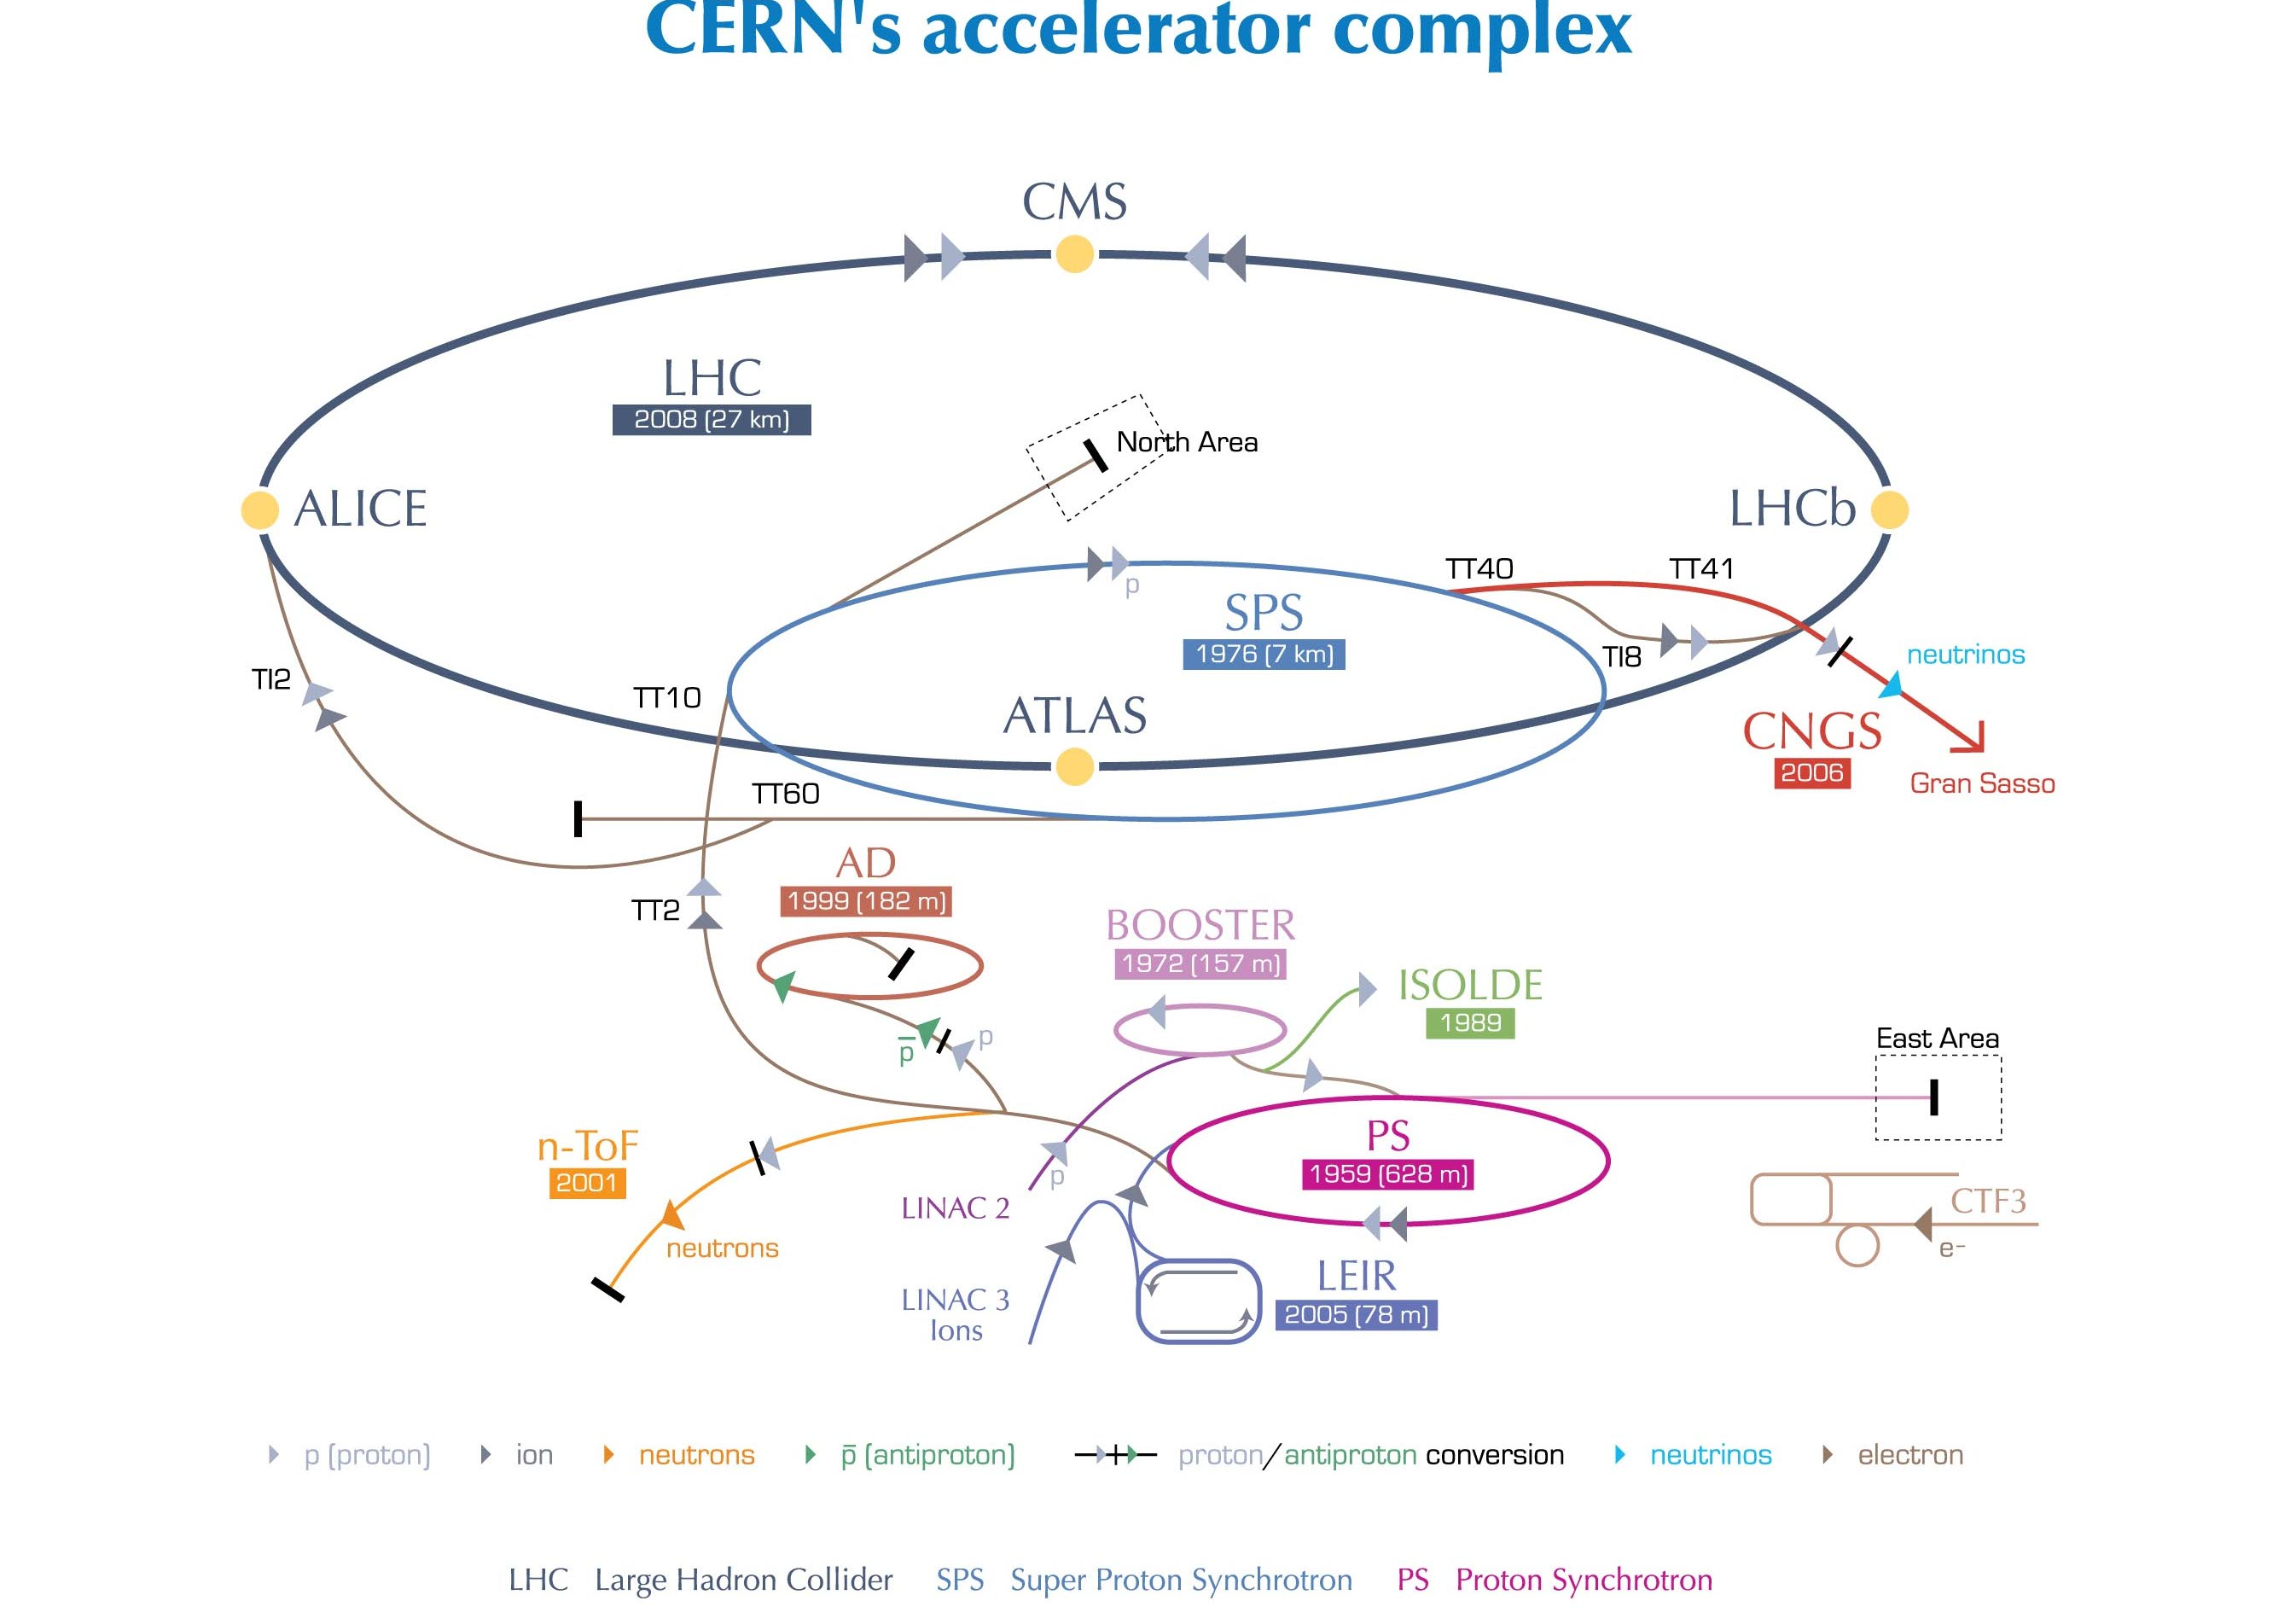
\includegraphics[width=0.95\textwidth]{images/LHCacc.jpg}
    \caption{The LHC accelerator complex at CERN}
    \label{fig:LHC acc}
\end{figure}


 The LHC was designed to have a centre of mass collision energy of $\sqrt{s} = 14 \TeV$. However, after an incident 10 days into operation in 2008 which caused damage to the LHC, it was restarted with the lower energy of $\sqrt{s} = 7 \TeV$ in 2011. In 2012 this was increased to $\sqrt{s} = 8 \TeV$ and a dataset with a \fixme*{luminosity}{explain lumi} of $\approx 20 \fbinv$ was recorded. This dataset was used for the analysis in chapter~\ref{c:Run1}. Further details on the run conditions can be found in \fixme{table of lumi, bunches etc.}. In 2013 after the run phase known as \emph{Run 1}, Long Shutdown 1 (LS1) commenced to make upgrades to the LHC and the detectors to allow the machine to run at $\sqrt{s} = 13 \TeV$ for \emph{Run 2}. Run 2 began in March 2015 and results from Run2 are the focus of the analysis in chapter~\ref{c:Run2}.

Run1 saw the great success of the discovery of the Higgs boson, one of the main objections of the LHC. In Run2, the search for new physics continues where precision measurements will test the predictions of the Standard Model.

\section{CMS detector}
\label{sec:CMSdet}

\subsection{Magnetic Solenoid}

\subsection{Tracker}

\subsection{Electromagnetic Calorimeter}

\subsection{Hadronic Calorimeter}

\subsection{Muon Chambers}

\subsection{Trigger}



\subsection{Upgrades for Run II}
